\section{Relational algebra in \dbsp}\label{sec:relational}

Results in \secref{sec:streams} and~\secref{sec:incremental}
apply to streams of arbitrary group values.  In this
section we turn our attention to using these results in the context of 
relational view maintenance.  As explained in the introduction, we want to
efficiently compute the incremental version of any relational query $Q$
that updates a database view.

However, we face a technical problem: the $\I$ and $\D$ operators were
defined on abelian groups, and relational databases in general are 
not abelian groups, since they operate on sets.  Fortunately, 
there is a well-known tool in the database literature
which converts set operations into group operations by using \zrs
(also called z-relations~\cite{green-pods07}) instead of sets.

We start by defining the \zrs group, and then we review how 
relational queries are converted into \dbsp circuits  over \zrs.  
What makes this translation incrementalizable is the fact that
many basic relational queries can be expressed using LTI \zr operators.

\subsection{\zrs as an abelian group}

Given a set $A$ we define \defined{\zrs}\footnote{Also called $\Z$-relations elsewhere~\cite{green-tcs11}.}
over $A$ as functions with \emph{finite support} from $A$ to $\Z$ (i.e., which are 0 almost everywhere).  
These are functions $f: A \rightarrow \Z$ where 
$f(x) \not= 0$ for at most a finite number of values $x \in A$.
We also write $\Z[A]$ for the type of \zrs with elements from $A$.
The values in $\Z[A]$ can also be thought as being key-value maps with 
keys in $A$ and values in $\Z$, justifying the array indexing notation.

Since $\Z$ is an abelian group, $\Z[A]$ is also an abelian group.  This group
$(\Z[A], +_{\Z[A]}, 0_{\Z[A]}, -_{\Z{A}})$ has addition and subtraction defined pointwise: 
$$(f +_{\Z[A]} g)(x) = f(x) + g(x) . \forall x \in A.$$  
The $0$ element of $\Z[A]$ is the function $0_{\Z[A]}$ defined by $0_{\Z[A]}(x) = 0 . \forall x \in A$. 
(In fact, since $\Z$ is a ring, $\Z[A]$ is also ring, endowed with a multiplication operation,
also defined pointwise.)

A particular \zr $m \in \Z[A]$ can be denoted by enumerating the inputs that map to non-zero values and
their multiplicities: 
$m = \{ x_1 \mapsto w_1, \dots, x_n \mapsto w_n \}$.  
We call $w_i \in Z$ the \defined{multiplicity} (or weight)
of $x_i \in A$.  Multiplicities can be negative.  
We write that $x \in m$ for $x \in A$, iff $m[x] \not= 0$.

For example, let's consider a concrete \zr $R \in \Z[\texttt{string}]$,
defined by $R = \{ \texttt{joe} \mapsto 1, \texttt{anne} \mapsto -1 \}$.  
$R$ has two elements in its domain,
\texttt{joe} with a multiplicity of 1 (so $R[\texttt{joe}] = 1$), 
and \texttt{anne} with a multiplicity of $-1$.
We say \texttt{joe} $\in R$ and \texttt{anne} $\in R$.

Given a \zr $m \in \Z[A]$ and a value $v \in A$, we overload the array index notation
$m[v]$ to denote the multiplicity of the element $v$ in $m$.  
Thus we write $R[\texttt{anne}] = -1$.
When $c \in \Z$, and $v \in A$ we also write $c \cdot v$ for the \defined{singleton} \zr $\{
v \mapsto c \}$.  In other words, $3 \cdot \texttt{frank} = \{ \texttt{frank} \mapsto 3 \}$.
We extend scalar multiplication to operate on \zrs: for $c \in Z, m \in \Z[A]$, 
$c \cdot m \defn \sum_{x \in m} (c \cdot m[x]) \cdot x$.  We then have
$2 \cdot R = \{ \texttt{joe} \mapsto 2, \texttt{anne} \mapsto -2 \}$: multiplying
each row weight by 2.

We define the \defined{size} of a \zr as the size of its support set, and we use the 
modulus symbol to represent the size: $|m| \defn \sum_{x \in m} 1$.  So $|R| = 2$.

\subsection{Sets, bags, and \zrs}

\zrs generalize sets and bags. 
Given a set with elements from $A$, it can be represented as a \zr $\Z[A]$ 
by associating a weight of 1 with each set element.  The function $\mbox{tozset}: 2^A \to \Z[A]$, 
defined as $\mbox{tozset}(s) = \sum_{x \in s} 1 \cdot x$, 
converts a set to a \zr by associating a multiplicity of 1 with each set element.
Thus $\mbox{tozset}(\{ \code{joe}, \code{anne} \}) = \{ \code{joe} \mapsto 1, \code{anne} \mapsto 1 \}$.

\begin{definition}
We say that a \zr represents a \defined{set} if the multiplicity of every
element is one.  We define a function to check this property 
$\isset : \Z[A] \rightarrow \B$\index{isset}, given by: 
$$\isset(m) \defn \left\{
\begin{array}{ll}
  \mbox{true} & \mbox{ if } m[x] = 1, \forall x \in m \\
  \mbox{false} & \mbox{ otherwise}
\end{array}
\right.
$$
\end{definition}
For our example $\isset(R) = \mbox{false}$, since $R[\texttt{anne}] = -1$.  
$\isset(\mbox{tozset}(m)) = \mbox{true}$ for any set $m \in 2^A$.

\begin{definition}
We say that a \zr is \defined{positive} (or a \defined{bag}) if the multiplicity of every element is
positive. We define a function to check this property
$\ispositive : \Z[A] \rightarrow \B$\index{ispositive}, given by
$$\ispositive(m) \defn \left\{
\begin{array}{ll}
  \mbox{true} & \mbox{ if } m[x] \geq 0, \forall x \in A \\
  \mbox{false} & \mbox{ otherwise}
\end{array}
\right.$$
\end{definition}
For our example $\ispositive(R) = \mbox{false}$, since $R[\texttt{anne}] = -1$,
but $\isset(m) \Rightarrow \ispositive(m). \forall m \in \Z[A]$.

We also write $m \geq 0$ when $m$ is
positive.  For positive $m, n$ we write $m \geq n$ for $m, n
\in \Z[A]$ iff $m - n \geq 0$.  The relation $\geq$ is a partial order.

\begin{definition}
The function $\distinct: \Z[A] \rightarrow \Z[A]$\index{distinct}
projects a \zr into an underlying set (but \emph{the result is
  still a \zr}).  The definition is $\forall x \in A$
$$\distinct(m)[x] \defn \left\{
\begin{array}{ll}
  1 & \mbox{ if } m[x] > 0 \\
  0 & \mbox{ otherwise}
\end{array}
\right.
$$
\end{definition}
$\distinct(R) = \{ \texttt{joe} \mapsto 1 \}$.

$\distinct$ ``removes'' elements with negative multiplicities.  $\zpp{\distinct}$.

Circuits derived from relational program will only operate with positive \zrs; 
non-positive values will be only used to represent \emph{changes} to \zrs 
(a change with negative weights will remove elements from a \zr).

\begin{proposition}
$\distinct$ is idempotent: $\distinct = \distinct \circ \distinct$.  
\end{proposition}

\begin{proposition}
For any $m \in \Z[A]$ we have: $\isset(\distinct(m))$ and \\
$\ispositive(\distinct(m))$.  
\end{proposition}

We call a function $f : \Z[I] \rightarrow \Z[O]$ \defined{positive} if
$\forall x \in \Z[I], x \geq 0_{\Z[I]} \Rightarrow f(x) \geq 0_{\Z[0]}$.  
We extend the notation used for \zrs for functions as well: $\ispositive(f)$.

\paragraph{Correctness of the \dbsp implementations}

The function $\mbox{toset}: \Z[A] \to 2^A$, defined as $\mbox{toset}(m) =
\cup_{x \in \distinct(m)} \{ x \}$, converts a \zr into a set.

A relational query $f$ that transforms
a set $V$ into a set $U$ will be implemented by a \dbsp computation $f'$ on 
\zrs.  The correctness of the implementation requires that the following
diagram commutes:

\begin{center}
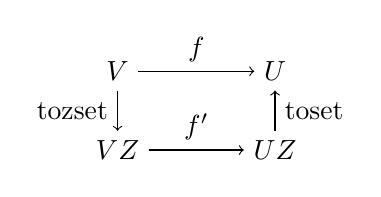
\begin{tikzpicture}
  \node[] (V) {$V$};
  \node[below of=V] (VZ) {$VZ$};
  \node[right of=V, node distance=2cm] (U) {$U$};
  \node[below of=U] (UZ) {$UZ$};
  \draw[->] (V) -- node (f) [above] {$f$} (U);
  \draw[->] (V) --  node (s) [left] {tozset}(VZ);
  \draw[->] (VZ) -- node (f) [above] {$f'$} (UZ);
  \draw[->] (UZ) -- node (d) [right] {toset} (U);
\end{tikzpicture}
\end{center}

\textbf{Remark:} We can generalize the notion of \zrs to functions $m: A \to \mathbf{G}$ for a
ring $\mathbf{G}$ other than $\Z$.  The properties we need from the ring structure are the
following: the ring must be a commutative group (needed for defining $\I$, $\D$, and $\zm$),
the multiplication operation must distribute over addition (needed to define 
Cartesian products), and there must be a notion of positive values, needed
to define the $\distinct$ function.  Rings such as $\mathbb{Q}$ or $\mathbb{R}$
would work perfectly.

\subsection{Streams over \zrs}

Since all the results from Section~\ref{sec:streams} are true for streams
over an arbitrary abelian group, they extend to streams where the elements 
are \zrs.  In the rest of this text we only consider streams of the form $\stream{\Z[A]}$, for
some element type $A$.

An example of a stream of \zrs is \\ $s = \sv{0 R -1\cdot{R} 2\cdot{R} -2\cdot{R}}$.
We have $s[2] = -R = \{ \texttt{joe} \mapsto -1, \texttt{anne} \mapsto 1 \}$.

\begin{definition}
A stream $s \in \stream{\Z[A]}$ is \defined{positive} if every value of the stream is positive:
$s[t] \geq 0 . \forall t \in \N$.
\end{definition}



\begin{definition}
A stream $s \in \stream{\Z[A]}$ is \defined{monotone} if $s[t] \geq s[t-1], \forall t \in \N$.
\end{definition}

\begin{lemma}
Given a positive stream $s \in \stream{\Z[A]}$ the stream $\I(s)$ is monotone.
\end{lemma}
\begin{proof}
  Let us compute $\I(s)[t + 1] - \I(s)[t] = \sum_{i \leq t+1}s[i] -
  \sum_{i \leq t}s[i] = s[t+1] \geq 0$, by commutativity and positivity of $s$.
\end{proof}

\begin{lemma}
Given a monotone stream $s \in \stream{\Z[A]}$, the
elements of the stream $\D(s)$ are positive.
\end{lemma}
\begin{proof}
  By the definition of monotonicity $s[t+1] \geq s[t]$.  By definition
  of $\D$ we have $\D(s)[t+1] = s[t+1] - s[t] \geq 0$.
\end{proof}

\subsection{Implementing the relational algebra}\label{sec:relational-operators}

The fact that the relational algebra can be implemented by computations
on \zrs has been shown before, e.g.~\cite{green-pods07}.  The translation
of the core relational operators is summarized in Table~\ref{tab:relational} and discussed below.

\begin{table*}
\begin{center}
\footnotesize
\begin{tabular}{|m{1.2cm}m{4.2cm}m{5cm}|} \hline
Operation & SQL example & \dbsp circuit  \\ \hline
Composition &
 \begin{lstlisting}[language=SQL]
SELECT DISTINCT ... FROM 
(SELECT ... FROM ...)
\end{lstlisting}
 & 
 \begin{tikzpicture}[auto,>=latex]
  \node[] (I) {\code{I}};
  \node[block, right of=I] (CI) {$C_I$};
  \draw[->] (I) -- (CI);
  \node[block, right of=CI] (CO) {$C_O$};
  \node[right of=CO] (O) {\code{O}};
  \draw[->] (CI) -- (CO);
  \draw[->] (CO) -- (O); 
\end{tikzpicture}
\\ \hline
Union & 
\begin{lstlisting}[language=SQL]
(SELECT * FROM I1) 
UNION 
(SELECT * FROM I2)
\end{lstlisting}
&
\begin{tikzpicture}[auto,>=latex]
  \node[] (input1) {\code{I1}};
  \node[below of=input1, node distance=.4cm] (midway) {};
  \node[below of=midway, node distance=.4cm] (input2) {\code{I2}};
  \node[block, shape=circle, right of=midway, inner sep=0in] (plus) {$+$};
  \node[block, right of=plus, node distance=1.5cm] (distinct) {$\distinct$};
  \node[right of=distinct, node distance=1.5cm] (output) {\code{O}};
  \draw[->] (input1) -| (plus);
  \draw[->] (input2) -| (plus);
  \draw[->] (plus) -- (distinct);
  \draw[->] (distinct) -- (output);
\end{tikzpicture}
\\ \hline
Projection &
\begin{lstlisting}[language=SQL]
SELECT DISTINCT I.c 
FROM I
\end{lstlisting}
&
\begin{tikzpicture}[auto,>=latex]
  \node[] (input) {\code{I}};
  \node[block, right of=input] (pi) {$\pi$};
  \node[block, right of=pi, node distance=1.5cm] (distinct) {$\distinct$};
  \node[right of=distinct, node distance=1.5cm] (output) {\code{O}};
  \draw[->] (input) -- (pi);
  \draw[->] (pi) -- (distinct);
  \draw[->] (distinct) -- (output);
\end{tikzpicture}
\\ \hline
Filtering &
\begin{lstlisting}[language=SQL]
SELECT * FROM I 
WHERE p(I.c)
\end{lstlisting}
&
\begin{tikzpicture}[auto,>=latex]
  \node[] (input) {\code{I}};
  \node[block, right of=input] (map) {$\sigma_P$};
  \node[block, right of=map, node distance=1.4cm] (distinct) {$\distinct$};
  \node[right of=distinct] (output) {\code{O}};
  \draw[->] (input) -- (map);
  \draw[->] (map) -- (distinct);
  \draw[->] (distinct) -- (output);
\end{tikzpicture}
\\ \hline
Selection &
\begin{lstlisting}[language=SQL]
SELECT DISTINCT f(I.c, ...) 
FROM I
\end{lstlisting}
&
\begin{tikzpicture}[auto,>=latex]
  \node[] (input) {\code{I}};
  \node[block, right of=input, node distance=1.5cm] (map) {$\mbox{map}(f)$};
  \node[block, right of=map, node distance=1.5cm] (distinct) {$\distinct$};
  \node[right of=distinct, node distance=1.5cm] (output) {\code{O}};
  \draw[->] (input) -- (map);
  \draw[->] (map) -- (distinct);
  \draw[->] (distinct) -- (output);
\end{tikzpicture}
\\ \hline
\parbox[b][][t]{1cm}{
Cartesian \\
product} &
\begin{lstlisting}[language=SQL]
SELECT I1.*, I2.* 
FROM I1, I2
\end{lstlisting}
& 
\begin{tikzpicture}[auto,>=latex]
  \node[] (i1) {\code{I1}};
  \node[below of=i1, node distance=.4cm] (midway) {};
  \node[below of=midway, node distance=.4cm] (i2) {\code{I2}};
  \node[block, right of=midway] (prod) {$\times$};
  \node[right of=prod] (output) {\code{O}};
  \draw[->] (i1) -| (prod);
  \draw[->] (i2) -| (prod);
  \draw[->] (prod) -- (output);
\end{tikzpicture}
\\ \hline
Join &
\begin{lstlisting}[language=SQL]
SELECT I1.*, I2.* 
FROM I1 JOIN I2
ON I1.c1 = I2.c2
\end{lstlisting}
&
\begin{tikzpicture}[auto,>=latex]
  \node[] (i1) {\code{I1}};
  \node[below of=i1, node distance=.4cm] (midway) {};
  \node[below of=midway, node distance=.4cm] (i2) {\code{I2}};
  \node[block, right of=midway] (prod) {$\bowtie$};
  \node[right of=prod] (output) {\code{O}};
  \draw[->] (i1) -| (prod);
  \draw[->] (i2) -| (prod);
  \draw[->] (prod) -- (output);
\end{tikzpicture}
\\ \hline
Intersection &
\begin{lstlisting}[language=SQL]
(SELECT * FROM I1)
INTERSECT 
(SELECT * FROM I2)
\end{lstlisting}
&
\begin{tikzpicture}[auto,>=latex]
  \node[] (i1) {\code{I1}};
  \node[below of=i1, node distance=.4cm] (midway) {};
  \node[below of=midway, node distance=.4cm] (i2) {\code{I2}};
  \node[block, right of=midway] (prod) {$\bowtie$};
  \node[right of=prod] (output) {\code{O}};
  \draw[->] (i1) -| (prod);
  \draw[->] (i2) -| (prod);
  \draw[->] (prod) -- (output);
\end{tikzpicture}
\\ \hline
Difference &
\begin{lstlisting}[language=SQL]
SELECT * FROM I1 
EXCEPT 
SELECT * FROM I2
\end{lstlisting}
&
\begin{tikzpicture}[auto,>=latex, node distance=.7cm]
  \node[] (i1) {\code{I1}};
  \node[below of=i1, node distance=.4cm] (midway) {};
  \node[below of=midway, node distance=.4cm] (i2) {\code{I2}};
  \node[block, shape=circle, inner sep=0in, right of=i2] (m) {$-$};
  \node[block, right of=midway, shape=circle, inner sep=0in, node distance=1.3cm] (plus) {$+$};
  \node[block, right of=plus, node distance=1.5cm] (distinct) {$\distinct$};
  \node[right of=distinct, node distance=1.5cm] (output) {\code{O}};
  \draw[->] (i1) -| (plus);
  \draw[->] (i2) -- (m);
  \draw[->] (m) -| (plus);
  \draw[->] (plus) -- (distinct);
  \draw[->] (distinct) -- (output);
\end{tikzpicture}
\\ \hline
\end{tabular}
\caption{Implementation of SQL relational set operators in \dbsp.  
Each query assumes that inputs \code{I}, \code{I1}, \code{I2}, are sets and it 
produces output sets.\label{tab:relational}}
\end{center}
\end{table*}

The translation is fairly straightforward, but many operators require
the application of a $\distinct$ to produce sets.  The correctness of
this implementation is predicated on the global circuit inputs being
sets as well. 

\subsubsection{Query composition}

A composite query is translated by compiling each sub-query separately into a circuit
and composing the respective circuits.

For example, consider the following SQL query:

\begin{lstlisting}[language=SQL]
SELECT ... FROM (SELECT ... FROM ...)
\end{lstlisting}

\noindent given circuits $C_O$ implementing the outer query and $C_I$
implementing the inner query, the translation of the composite query is:

\begin{center}
\begin{tikzpicture}[auto,>=latex]
  \node[] (I) {\code{I}};
  \node[block, right of=I] (CI) {$C_I$};
  \draw[->] (I) -- (CI);
  \node[block, right of=CI] (CO) {$C_O$};
  \node[right of=CO] (O) {\code{O}};
  \draw[->] (CI) -- (CO);
  \draw[->] (CO) -- (O); 
\end{tikzpicture}
\end{center}

We have $\ispositive(C_I) \land \ispositive(C_0) \Rightarrow \ispositive(C_O \circ C_I)$
and $\zpp{C_I} \land \zpp{C_O} \Rightarrow \zpp{C_O \circ C_I}$.

\subsubsection{Set union}

Consider the following SQL query:

\begin{lstlisting}[language=SQL]
(SELECT * FROM I1) UNION (SELECT * FROM I2)
\end{lstlisting}

The following circuit implements the union program:

\begin{center}
\begin{tikzpicture}[auto,>=latex]
  \node[] (input1) {\code{I1}};
  \node[below of=input1, node distance=.4cm] (midway) {};
  \node[below of=midway, node distance=.4cm] (input2) {\code{I2}};
  \node[block, shape=circle, right of=midway, inner sep=0in] (plus) {$+$};
  \node[block, right of=plus, node distance=1.5cm] (distinct) {$\distinct$};
  \node[right of=distinct, node distance=1.5cm] (output) {\code{O}};
  \draw[->] (input1) -| (plus);
  \draw[->] (input2) -| (plus);
  \draw[->] (plus) -- (distinct);
  \draw[->] (distinct) -- (output);
\end{tikzpicture}
\end{center}

Given \zrs $a, b \in \Z[I]$ s.t. $\isset(a)$ and $\isset(b)$, their \emph{set union} 
can be computed as: $\cup: \Z[I] \times \Z[I] \rightarrow \Z[I]$,  $$a
\cup b \defn \distinct(a +_{\Z[I]} b).$$  
The $\distinct$ application is necessary to provide the set semantics.

\subsubsection{Projection}
Consider a query such as:

\begin{lstlisting}[language=SQL]
SELECT I.c FROM I
\end{lstlisting}

We can assume without loss of generality that table \code{I} has two columns, and that 
a single column is preserved in the projection.
Hence the type of \code{I} is $\Z[A_0 \times A_1]$ while the result has type is $\Z[A_0]$.
In terms of \zrs, the projection of a \zr $i$ on $A_0$ is defined as: $$\pi(i)[y] = 
\sum_{x \in i, x|_0 = y} i[x]$$
\noindent where $x|_0$ is first component of the tuple $x$.
In other words, the multiplicity of a tuple in the result is the sum 
of the multiplicities of all input tuples that project to it.

The circuit for a projection query is:

\begin{center}
\begin{tikzpicture}[auto,>=latex]
  \node[] (input) {\code{I}};
  \node[block, right of=input] (pi) {$\pi$};
  \node[block, right of=pi, node distance=1.5cm] (distinct) {$\distinct$};
  \node[right of=distinct, node distance=1.5cm] (output) {\code{O}};
  \draw[->] (input) -- (pi);
  \draw[->] (pi) -- (distinct);
  \draw[->] (distinct) -- (output);
\end{tikzpicture}
\end{center}

The $\distinct$ is necessary to convert the result to a set.\\
$\pi$ is linear; $\ispositive(\pi), \zpp{\pi}$.

\subsubsection{Selection}

We generalize the SQL selection operator to allow it to apply an arbitrary function to each row of the
selected set.
Given a function $f : A \rightarrow B$, the mathematical \defined{map} operator ``lifts'' the
function $f$ to operate on \zrs: $\map(f) : \Z[A] \rightarrow \Z[B]$.  A map operator
appears in SQL due to the use of expressions in the SELECT clause, as in the following example:

\begin{lstlisting}[language=SQL]
SELECT f(I.c) FROM I
\end{lstlisting}

The circuit implementation of this query is:

\begin{center}
\begin{tikzpicture}[auto,>=latex]
  \node[] (input) {\code{I}};
  \node[block, right of=input, node distance=1.5cm] (map) {$\mbox{map}(f)$};
  \node[block, right of=map, node distance=2cm] (distinct) {$\distinct$};
  \node[right of=distinct, node distance=1.5cm] (output) {\code{O}};
  \draw[->] (input) -- (map);
  \draw[->] (map) -- (distinct);
  \draw[->] (distinct) -- (output);
\end{tikzpicture}
\end{center}

For any function $f$ we have the following properties:
$\map(f)$ is linear, $\ispositive(\map(f)), and \zpp{\map(f)}.$

\subsubsection{Filtering}

Filtering occurs in SQL through a WHERE clause, as in the following example:

\noindent
\begin{lstlisting}[language=SQL]
SELECT * FROM I WHERE p(I.c)
\end{lstlisting}

Let us assume that we are filtering with a predicate 
$P: A \rightarrow \B$.  We define the following function $\sigma_P: \Z[A] \rightarrow \Z[A]$ as:
$$\sigma_P(m)[t] = \left\{
\begin{array}{ll}
  m[t] \cdot t & \mbox{ if } P(t) \\
  0 & \mbox{ otherwise } \\
\end{array}
\right.
$$

The circuit for filtering with a predicate $P$ is:

\begin{center}
\begin{tikzpicture}[auto,>=latex]
  \node[] (input) {\code{I}};
  \node[block, right of=input] (map) {$\sigma_P$};
  \node[right of=map] (output) {\code{O}};
  \draw[->] (input) -- (map);
  \draw[->] (map) -- (output);
\end{tikzpicture}
\end{center}

For any predicate $P$ we have $\isset(i) \Rightarrow
\isset(\sigma_P(i))$ and $\ispositive(\sigma_P)$.  Thus a $\distinct$
is not needed.  $\sigma_P$ is linear and $\zpp{\sigma_P}$.

\subsubsection{Cartesian products}

Consider this SQL query performing a Cartesian product
between sets \code{I1} and \code{I2}:

\begin{lstlisting}[language=SQL]
SELECT I1.*, I2.* FROM I1, I2
\end{lstlisting}

We first define a product operation on \zrs.
For $a \in \Z[A]$ and $b \in \Z[B]$ we define $a \times b \in \Z[A \times B]$ by
$$(a \times b)((x,y)) \defn a[x] \times b[y] . \forall x \in a, y \in b.$$
The weight of a pair in the result is the product of the weights of the 
elements in the sources.  The circuit for the query is:

\begin{center}
\begin{tikzpicture}[auto,>=latex]
  \node[] (i1) {\code{I1}};
  \node[below of=i1, node distance=.5cm] (midway) {};
  \node[below of=midway, node distance=.5cm] (i2) {\code{I2}};
  \node[block, right of=midway] (prod) {$\times$};
  \node[right of=prod] (output) {\code{O}};
  \draw[->] (i1) -| (prod);
  \draw[->] (i2) -| (prod);
  \draw[->] (prod) -- (output);
\end{tikzpicture}
\end{center}

$\isset(x) \land \isset(y) \Rightarrow \isset(x \times y).$
$\times$ is bilinear, $\ispositive(\times), \zpp{\times}$.

\subsubsection{Joins}

As is well-known, joins can be modeled as Cartesian products
followed by filtering.  Since a join is a composition of a bilinear 
and a linear operator, it is also a bilinear operator.
$\ispositive(\bowtie), \zpp{\bowtie}.$

In practice joins are very important computationally, and they are
implemented by a built-in scalar function on \zrs:

$$(a \bowtie b)((x,y)) \defn a[x] \times b[y] \mbox{ if } x|_{c1} = y|_{c2}.$$

\begin{center}
\begin{tikzpicture}[auto,>=latex]
  \node[] (i1) {\code{I1}};
  \node[below of=i1, node distance=.5cm] (midway) {};
  \node[below of=midway, node distance=.5cm] (i2) {\code{I2}};
  \node[block, right of=midway] (prod) {$\bowtie$};
  \node[right of=prod] (output) {\code{O}};
  \draw[->] (i1) -| (prod);
  \draw[->] (i2) -| (prod);
  \draw[->] (prod) -- (output);
\end{tikzpicture}
\end{center}

\subsubsection{Set intersection}

Set intersection is a special case of join, where both relations have the same schema.
It follows that set intersection is bilinear,
and has the zero-preservation property.

\subsubsection{Set difference}  Consider the following query:

\begin{lstlisting}[language=SQL]
SELECT * FROM I1 EXCEPT SELECT * FROM I2
\end{lstlisting}

We define the set difference on \zrs as follows: 
$\setminus: \Z[I] \times \Z[I] \rightarrow \Z[I]$, where $$i_1
\setminus i_2 = \distinct(i_1 - i_2).$$  Note
that we have $\forall i_1, i_2, \ispositive(i_1 \setminus
i_2)$ due to the $\distinct$ operator.
The circuit computing the above query is:

\begin{center}
\begin{tikzpicture}[auto,>=latex, node distance=.7cm]
  \node[] (i1) {\code{I1}};
  \node[below of=i1, node distance=.4cm] (midway) {};
  \node[below of=midway, node distance=.4cm] (i2) {\code{I2}};
  \node[block, shape=circle, inner sep=0in, right of=i2] (m) {$-$};
  \node[block, right of=midway, shape=circle, inner sep=0in, node distance=1.3cm] (plus) {$+$};
  \node[block, right of=plus, node distance=1.5cm] (distinct) {$\distinct$};
  \node[right of=distinct, node distance=1.5cm] (output) {\code{O}};
  \draw[->] (i1) -| (plus);
  \draw[->] (i2) -- (m);
  \draw[->] (m) -| (plus);
  \draw[->] (plus) -- (distinct);
  \draw[->] (distinct) -- (output);
\end{tikzpicture}
\end{center}

\subsection{Optimizing relational circuits}

\subsubsection{Optimizing $\distinct$}

All standard algebraic properties
of the relational operators can be used to optimize circuits.  In addition,
a few optimizations are related to the $\distinct$ operator, which is
not linear, and thus expensive to incrementalize:

\begin{proposition}\label{prop-distinct-delay}
Let Q be one of the following \zrs operators: filtering $\sigma$,
join $\bowtie$, or Cartesian product $\times$.
Then we have $\forall i \in \Z[I], \ispositive(i) \Rightarrow Q(\distinct(i)) = \distinct(Q(i))$.
\end{proposition}

\begin{center}
\begin{tabular}{m{3.5cm}m{.5cm}m{3.5cm}}
\begin{tikzpicture}[auto,>=latex]
  \node[] (input) {$i$};
  \node[block, right of=input, node distance=1.1cm] (distinct) {$\distinct$};
  \node[block, right of=distinct, node distance=1.2cm] (q) {$Q$};
  \node[right of=q] (output)  {$o$};
  \draw[->] (input) -- (distinct);
  \draw[->] (distinct) -- (q);
  \draw[->] (q) -- (output);
\end{tikzpicture}
&
$\cong$
&
\begin{tikzpicture}[auto,>=latex]
  \node[] (input) {$i$};
  \node[block, right of=input] (q) {$Q$};
  \node[block, right of=q, node distance=1.2cm] (distinct1) {$\distinct$};
  \node[right of=distinct1, node distance=1.2cm] (output)  {$o$};
  \draw[->] (input) -- (q);
  \draw[->] (q) -- (distinct1);
  \draw[->] (distinct1) -- (output);
\end{tikzpicture}
\end{tabular}
\end{center}

This rule allows us to delay the application of $\distinct$.

\begin{proposition}\label{prop-distinct-once}
Let Q be one of the following \zrs operators: filtering $\sigma$,
projection $\pi$, selection (map($f$)), addition $+$, join $\bowtie$, or
Cartesian product $\times$.
Then we have $\forall i \in \Z[I], \ispositive(i) \Rightarrow \distinct(Q(\distinct(i))) = \distinct(Q(i))$.
\end{proposition}

This is Proposition 6.13 in~\cite{green-tcs11}.

\begin{center}
\begin{tabular}{m{6.5cm}m{.5cm}}
\begin{tikzpicture}[auto,>=latex]
  \node[] (input) {$i$};
  \node[block, right of=input, node distance=1.5cm] (distinct) {$\distinct$};
  \node[block, right of=distinct, node distance=1.5cm] (q) {$Q$};
  \node[block, right of=q, node distance=1.5cm] (distinct1) {$\distinct$};
  \node[right of=distinct1, node distance=1.5cm] (output)  {$o$};
  \draw[->] (input) -- (distinct);
  \draw[->] (distinct) -- (q);
  \draw[->] (q) -- (distinct1);
  \draw[->] (distinct1) -- (output);
\end{tikzpicture}
&
$\cong$ \\
\begin{tikzpicture}[auto,>=latex]
  \node[] (input) {$i$};
  \node[block, right of=input] (q) {$Q$};
  \node[block, right of=q, node distance=1.5cm] (distinct1) {$\distinct$};
  \node[right of=distinct1, node distance=1.5cm] (output)  {$o$};
  \draw[->] (input) -- (q);
  \draw[->] (q) -- (distinct1);
  \draw[->] (distinct1) -- (output);
\end{tikzpicture}
\end{tabular}
\end{center}

These properties allow us to ``consolidate'' distinct operators by performing
one distinct at the end of a chain of computations.

\begin{proposition}\label{inc_distinct}
The following circuit implements $\inc{(\lift{\distinct})}$:

\begin{center}
\begin{tabular}{m{3.5cm}m{.5cm}m{6cm}}
\begin{tikzpicture}[auto,node distance=1.5cm,>=latex]
    \node[] (input) {$d$};
    \node[block, right of=input] (d) {$\inc{(\lift{\distinct})}$};
    \node[right of=d] (output) {$o$};
    \draw[->] (input) -- (d);
    \draw[->] (d) -- (output);
\end{tikzpicture} &
$\cong$ &
\begin{tikzpicture}[>=latex]
    \node[] (input) {$d$};
    \node[block, right of=input] (I) {$\I$};
    \node[block, right of=I] (z) {$\zm$};
    \node[block, below of=z, node distance=1cm] (H) {$\lift{H}$};
    \node[right of=H] (output) {$o$};
    \draw[->] (input) -- node (mid) {} (I);
    \draw[->] (I) -- (z);
    \draw[->] (mid.center) |- (H);
    \draw[->] (z) -- node (i) [right] {$i$} (H);
    \draw[->] (H) -- (output);
\end{tikzpicture}
\end{tabular}
\end{center}

\noindent where $H: \Z[A] \times \Z[A] \to \Z[A]$ is defined as:
$$
H(i, d)[x] \defn 
\begin{cases}
-1 & \mbox{if } i[x] > 0 \mbox{ and } (i + d)[x] \leq 0 \\
1  & \mbox{if } i[x] \leq 0 \mbox{ and } (i + d)[x] > 0 \\
0  & \mbox{otherwise} \\
\end{cases}
$$
\end{proposition}

The function $H$ detects whether the multiplicity of an element in the 
input set $i$ is changing from negative to positive or vice-versa. 

\subsubsection{Anti-joins}

TODO\mihai{justify this.}

\begin{tikzpicture}[auto,>=latex]
  \node[] (i1) {\code{I1}};
  \node[below of=i1, node distance=.7cm] (i2) {\code{I2}};
  \node[block, right of=i1, node distance=1.5cm] (join) {$\bowtie$};
  \node[block, shape=circle, inner sep=0in, right of=join] (m) {$-$};
  \node[block, above of=m, shape=circle, inner sep=0in, node distance=.7cm] (plus) {$+$};
  \node[block, right of=plus, node distance=1.5cm] (distinct) {$\distinct$};
  \node[right of=distinct, node distance=1.5cm] (output) {\code{O}};
  \draw[->] (i1) -- node (tap) {} (join);
  \draw[->] (i2) -| (join);
  \draw[->] (join) -- (m);
  \draw[->] (m) -- (plus);
  \draw[->] (tap.south) |- (plus);
  \draw[->] (plus) -- (distinct);
  \draw[->] (distinct) -- (output);
\end{tikzpicture}

This can be optimized as follows:

\begin{tikzpicture}[auto,>=latex]
  \node[] (i1) {\code{I1}};
  \node[below of=i1, node distance=.7cm] (i2) {\code{I2}};
  \node[block, right of=i2, node distance=1.5cm] (distinct) {$\distinct$};
  \node[block, shape=circle, inner sep=0in, right of=distinct, node distance=1.5cm] (m) {$-$};
  \node[block, above of=m, node distance=.7cm] (join) {$\bowtie$};
  \node[block, above of=join, shape=circle, inner sep=0in, node distance=.7cm] (plus) {$+$};
  \node[right of=plus, node distance=1.5cm] (output) {\code{O}};
  \draw[->] (i1) -- node (tap) {} (join);
  \draw[->] (i2) -- (distinct);
  \draw[->] (distinct) -- (m);
  \draw[->] (m) -- (join);
  \draw[->] (join) -- (plus);
  \draw[->] (tap.south) |- (plus);
  \draw[->] (plus) -- (output);
\end{tikzpicture}

\subsection{Parallelization}

DBSP is rich enough to express operators such as the Volcano exchange
operator~\cite{graefe-sigmod90}, which can be used to parallelize DBSP circuits.
The following circuit shows a parallel implementation of a join operator.

\begin{tabular}{m{2.5cm}m{.7cm}m{5cm}}
\begin{tikzpicture}
\node[] (s1) {$s_1$};
\node[below of=i1, node distance=1.5cm] (s2) {$s_2$};
\node[right of=s1] (invisible) {};
\node[below of=invisible, block, node distance=.75cm] (join) {$\bowtie$};
\draw[->] (s1) -| (join);
\draw[->] (s2) -| (join);
\node[right of=join] (o) {$o$};
\draw[->] (join) -- (o);
\end{tikzpicture}
     &  
     $\cong$
     & 
\begin{tikzpicture}
\node[] (s1) {$s_1$};
\node[right of=s1, block] (s1s) {};
\node[right of=s1s] (invisible1) {};
\node[above of=invisible1, block, node distance=.5cm] (sigma11) {$\sigma_1$};
\node[below of=invisible1, block, node distance=.5cm] (sigma12) {$\sigma_2$};

\node[below of=i1, node distance=1.5cm] (s2) {$s_2$};
\node[right of=s2, block] (s2s) {};
\node[right of=s2s] (invisible2) {};
\node[above of=invisible2, block, node distance=.5cm] (sigma21) {$\sigma_1$};
\node[below of=invisible2, block, node distance=.5cm] (sigma22) {$\sigma_2$};
\draw[->] (s1) -- (s1s);
\draw[->] (s1s) |- (sigma11);
\draw[->] (s1s) |- (sigma12);

\draw[->] (s2) -- (s2s);
\draw[->] (s2s) |- (sigma21);
\draw[->] (s2s) |- (sigma22);

\node[block, right of=invisible1, node distance=1.5cm] (join1) {$\bowtie$};
\node[block, right of=invisible2, node distance=2cm] (join2) {$\bowtie$};
\node[block, right of=join1, shape=circle, inner sep=0in] (plus) {$+$}; 
\node[right of=plus] (o) {$o$};

\draw[->] (sigma11) -| (join1);
\draw[->] (sigma21) -| (join1);
\draw[->] (sigma12) -| (join2);
\draw[->] (sigma22) -| (join2);
\draw[->] (join1) -- (plus);
\draw[->] (join2) -| (plus);
\draw[->] (plus) -- (o);

\end{tikzpicture}
\end{tabular}

Here is an example of an exchange operator which repartitions the data
in a collection from two partitions to three partitions, where $\sigma_i$ 
for $i \in [3]$ are disjoint selection functions that partition the space
of tuples.

\begin{tikzpicture}[auto,>=latex]
  \node[] (s1) {$s_1$};
  \node[below of=i1, node distance=2cm] (s2) {$s_2$};
  \node[block, right of=s1] (s12) {$\sigma_2$};
  \node[block, above of=s12, node distance=.7cm] (s11) {$\sigma_1$};
  \node[block, below of=s12, node distance=.7cm] (s13) {$\sigma_3$};
  \draw[->] (s1) -- node(mid) {} (s12);
  \draw[->] (mid.south) |- (s11);
  \draw[->] (mid) |- (s13);
  \node[block, right of=s2] (s22) {$\sigma_2$};
  \node[block, above of=s22, node distance=.7cm] (s21) {$\sigma_1$};
  \node[block, below of=s22, node distance=.7cm] (s23) {$\sigma_3$};
  \draw[->] (s2) -- node(mid2) {} (s22);
  \draw[->] (mid2.south) |- (s21);
  \draw[->] (mid2) |- (s23);
  \node[block, right of=s11, node distance=1cm, shape=circle, inner sep=0in] (p1) {$+$};
  \node[block, right of=s12, node distance=1.5cm, shape=circle, inner sep=0in] (p2) {$+$};
  \node[block, right of=s13, node distance=2cm, shape=circle, inner sep=0in] (p3) {$+$};
  \draw[->] (s11) -- (p1);
  \draw[->] (s12) -- (p2);
  \draw[->] (s13) -- (p3);
  \draw[->] (s21) -| (p1);
  \draw[->] (s22) -| (p2);
  \draw[->] (s23) -| (p3);
  \node[right of=p1] (o1) {$o_1$};
  \node[right of=p2] (o2) {$o_2$};
  \node[right of=p3] (o3) {$o_3$};
  \draw[->] (p1) -- (o1);
  \draw[->] (p2) -- (o2);
  \draw[->] (p3) -- (o3);
\end{tikzpicture}

\subsection{Incremental relational queries}\label{sec:incremental-relational}

Let us consider a relational query $Q$ 
defining a view.  To create a circuit that maintains incrementally the view defined by $Q$
we apply the following mechanical steps:

\begin{algorithm}[incremental view maintenance]\label{algorithm-inc}\quad
\begin{enumerate}
    \item Translate $Q$ into a circuit using the rules in Table~\ref{tab:relational}.
    \item Apply optimization rules, including $\distinct$ consolidation.
    \item Lift the whole circuit, by applying Proposition~\ref{prop:distributivity},
    converting it to a circuit operating on streams.
    \item Incrementalize the whole circuit ``surrounding'' it with $\I$ and $\D$.
    \item Apply the chain rule and other properties of the $\inc{\cdot}$ operator
    from Proposition~\ref{prop-inc-properties} to optimize the incremental implementation.
\end{enumerate}
\end{algorithm}

Step (3) yields a circuit that consumes a stream of complete database snapshots and outputs a 
stream of complete view snapshots. Step (4) yields a circuit that consumes a stream of changes
to the database and outputs a stream of view changes; however, the internal operation of the 
circuit is non-incremental, as it computes on the complete state of the database reconstructed
by the integration operator.  Step (5) incrementalizes the internals of the circuit by rewriting 
it to compute on changes, avoiding integration when possible (see \secref{sec:incremental}).

\subsubsection{Examples}

In this section we apply the incremental view maintenance algorithm to a concrete
query.  Let us consider the following query:

\begin{lstlisting}[language=SQL]
CREATE VIEW v AS
SELECT DISTINCT t1.x, t2.y FROM (
     SELECT t1.x, t1.id 
     FROM t 
     WHERE t.a > 2 
) t1  
JOIN (
     SELECT t2.id, t2.y
     FROM r 
     WHERE r.s > 5 
) t2 ON t1.id = t2.id
\end{lstlisting}

Step 1: First we create a \dbsp circuit to represent this query using the
translation rules from Table~\ref{tab:relational}:

\noindent
\begin{tikzpicture}[node distance=1.5cm,>=latex]
    \node[] (t1) {\code{t1}};
    \node[block, right of=t1, node distance=1.2cm] (s1) {$\sigma_{a > 2}$};
    \node[block, right of=s1] (d1) {$\distinct$};
    \node[block, right of=d1] (p1) {$\pi_{x, id}$};
    \node[block, right of=p1] (d11) {$\distinct$};
    \node[below of=t1, node distance=1cm] (t2) {\code{t2}};
    \node[block, right of=t2, node distance=1.2cm] (s2) {$\sigma_{s > 5}$};
    \node[block, right of=s2] (d2) {$\distinct$};
    \node[block, right of=d2] (p2) {$\pi_{id, y}$};
    \node[block, right of=p2] (d21) {$\distinct$};
    \node[below of=d11, node distance=.5cm] (mid) {};
    \node[block, right of=mid] (j) {$\bowtie_{id = id}$};
    \node[block, right of=j] (p) {$\pi_{x, y}$};
    \node[block, right of=p] (d) {$\distinct$};
    \node[right of=d, node distance=1.2cm] (V) {\code{V}};
    \draw[->] (t1) -- (s1);
    \draw[->] (s1) -- (d1);
    \draw[->] (d1) -- (p1);
    \draw[->] (p1) -- (d11);
    \draw[->] (t2) -- (s2);
    \draw[->] (s2) -- (d2);
    \draw[->] (d2) -- (p2);
    \draw[->] (p2) -- (d21);
    \draw[->] (d11) -| (j);
    \draw[->] (d21) -| (j);
    \draw[->] (j) -- (p);
    \draw[->] (p) -- (d);
    \draw[->] (d) -- (V);
\end{tikzpicture}

Step 2: we apply the $\distinct$ optimization rules; first the rule from~\ref{prop-distinct-once}
gives us the following equivalent circuit:

\noindent
\begin{tikzpicture}[node distance=1.5cm,>=latex]
    \node[] (t1) {\code{t1}};
    \node[block, right of=t1, node distance=1.2cm] (s1) {$\sigma_{a > 2}$};
    \node[block, right of=s1] (p1) {$\pi_{x, id}$};
    \node[block, right of=p1] (d11) {$\distinct$};
    \node[below of=t1, node distance=1cm] (t2) {\code{t2}};
    \node[block, right of=t2, node distance=1.2cm] (s2) {$\sigma_{s > 5}$};
    \node[block, right of=s2] (p2) {$\pi_{id, y}$};
    \node[block, right of=p2] (d21) {$\distinct$};
    \node[below of=d11, node distance=.5cm] (mid) {};
    \node[block, right of=mid, node distance=1.2cm] (j) {$\bowtie_{id = id}$};
    \node[block, right of=j] (p) {$\pi_{x, y}$};
    \node[block, right of=p] (d) {$\distinct$};
    \node[right of=d, node distance=1.2cm] (V) {\code{V}};
    \draw[->] (t1) -- (s1);
    \draw[->] (s1) -- (p1);
    \draw[->] (p1) -- (d11);
    \draw[->] (t2) -- (s2);
    \draw[->] (s2) -- (p2);
    \draw[->] (p2) -- (d21);
    \draw[->] (d11) -| (j);
    \draw[->] (d21) -| (j);
    \draw[->] (j) -- (p);
    \draw[->] (p) -- (d);
    \draw[->] (d) -- (V);
\end{tikzpicture}

Applying the rule from~\ref{prop-distinct-delay} we get:

\noindent
\begin{tikzpicture}[node distance=1.5cm,>=latex]
    \node[] (t1) {\code{t1}};
    \node[block, right of=t1, node distance=.9cm] (s1) {$\sigma_{a > 2}$};
    \node[block, right of=s1] (p1) {$\pi_{x, id}$};
    \node[below of=t1, node distance=1cm] (t2) {\code{t2}};
    \node[block, right of=t2, node distance=.9cm] (s2) {$\sigma_{s > 5}$};
    \node[block, right of=s2] (p2) {$\pi_{id, y}$};
    \node[below of=p1, node distance=.5cm] (mid) {};
    \node[block, right of=mid, node distance=1.2cm] (j) {$\bowtie_{id = id}$};
    \node[block, right of=j, node distance=1.7cm] (d0) {$\distinct$};
    \node[block, right of=d0] (p) {$\pi_{x, y}$};
    \node[block, right of=p] (d) {$\distinct$};
    \node[right of=d, node distance=1.2cm] (V) {\code{V}};
    \draw[->] (t1) -- (s1);
    \draw[->] (s1) -- (p1);
    \draw[->] (t2) -- (s2);
    \draw[->] (s2) -- (p2);
    \draw[->] (p1) -| (j);
    \draw[->] (p2) -| (j);
    \draw[->] (j) -- (d0);
    \draw[->] (d0) -- (p);
    \draw[->] (p) -- (d);
    \draw[->] (d) -- (V);
\end{tikzpicture}

And applying again~\ref{prop-distinct-once} we get:

\noindent
\begin{tikzpicture}[node distance=1.5cm,>=latex]
    \node[] (t1) {\code{t1}};
    \node[block, right of=t1, node distance=.9cm] (s1) {$\sigma_{a > 2}$};
    \node[block, right of=s1] (p1) {$\pi_{x, id}$};
    \node[below of=t1, node distance=1cm] (t2) {\code{t2}};
    \node[block, right of=t2, node distance=.9cm] (s2) {$\sigma_{s > 5}$};
    \node[block, right of=s2] (p2) {$\pi_{id, y}$};
    \node[below of=p1, node distance=.5cm] (mid) {};
    \node[block, right of=mid, node distance=1.2cm] (j) {$\bowtie_{id = id}$};
    \node[block, right of=j] (p) {$\pi_{x, y}$};
    \node[block, right of=p] (d) {$\distinct$};
    \node[right of=d, node distance=1.2cm] (V) {\code{V}};
    \draw[->] (t1) -- (s1);
    \draw[->] (s1) -- (p1);
    \draw[->] (t2) -- (s2);
    \draw[->] (s2) -- (p2);
    \draw[->] (p1) -| (j);
    \draw[->] (p2) -| (j);
    \draw[->] (j) -- (p);
    \draw[->] (p) -- (d);
    \draw[->] (d) -- (V);
\end{tikzpicture}

Step 3: we lift the circuit using distributivity of composition over lifting; we
obtain a circuit that computes over streams, i.e., for each new input pair of relations
\code{t1} and \code{t2} it will produce an output view \code{V}:

\noindent
\begin{tikzpicture}[node distance=1.7cm,>=latex]
    \node[] (t1) {\code{t1}};
    \node[block, right of=t1, node distance=1.1cm] (s1) {$\lift{\sigma_{a > 2}}$};
    \node[block, right of=s1] (p1) {$\lift{\pi_{x, id}}$};
    \node[below of=t1, node distance=1.2cm] (t2) {\code{t2}};
    \node[block, right of=t2, node distance=1.1cm] (s2) {$\lift{\sigma_{s > 5}}$};
    \node[block, right of=s2] (p2) {$\lift{\pi_{id, y}}$};
    \node[below of=p1, node distance=.6cm] (mid) {};
    \node[block, right of=mid, node distance=1.3cm] (j) {$\lift{\bowtie_{id = id}}$};
    \node[block, right of=j] (p) {$\lift{\pi_{x, y}}$};
    \node[block, right of=p] (d) {$\lift{\distinct}$};
    \node[right of=d] (V) {\code{V}};
    \draw[->] (t1) -- (s1);
    \draw[->] (s1) -- (p1);
    \draw[->] (t2) -- (s2);
    \draw[->] (s2) -- (p2);
    \draw[->] (p1) -| (j);
    \draw[->] (p2) -| (j);
    \draw[->] (j) -- (p);
    \draw[->] (p) -- (d);
    \draw[->] (d) -- (V);
\end{tikzpicture}

Step 4: incrementalize circuit, obtaining a circuit that computes over changes;
this circuit receives changes to relations \code{t1} and \code{t2} and for each
such change it produces the corresponding change in the output view \code{V}:

\noindent
\begin{tikzpicture}[node distance=1.7cm,>=latex]
    \node[] (t1) {$\Delta$\code{t1}};
    \node[block, right of=t1, node distance=.8cm] (I1) {$\I$};
    \node[block, right of=I1, node distance=1.3cm] (s1) {$\lift{\sigma_{a > 2}}$};
    \node[block, right of=s1] (p1) {$\lift{\pi_{x, id}}$};
    \node[below of=t1, node distance=1.2cm] (t2) {$\Delta$\code{t2}};
    \node[block, right of=t2, node distance=.8cm] (I2) {$\I$};
    \node[block, right of=I2, node distance=1.3cm] (s2) {$\lift{\sigma_{s > 5}}$};
    \node[block, right of=s2] (p2) {$\lift{\pi_{id, y}}$};
    \node[below of=p1, node distance=.6cm] (mid) {};
    \node[block, right of=mid, node distance=1.6cm] (j) {$\lift{\bowtie_{id = id}}$};
    \node[block, right of=j] (p) {$\lift{\pi_{x, y}}$};
    \node[block, right of=p] (d) {$\lift{\distinct}$};
    \node[block, right of=d, node distance=1.3cm] (D) {$\D$};
    \node[right of=D, node distance=1.2cm] (V) {$\Delta$\code{V}};
    \draw[->] (t1) -- (I1);
    \draw[->] (I1) -- (s1);
    \draw[->] (s1) -- (p1);
    \draw[->] (t2) -- (I2);
    \draw[->] (I2) -- (s2);
    \draw[->] (s2) -- (p2);
    \draw[->] (p1) -| (j);
    \draw[->] (p2) -| (j);
    \draw[->] (j) -- (p);
    \draw[->] (p) -- (d);
    \draw[->] (d) -- (D);
    \draw[->] (D) -- (V);
\end{tikzpicture}

Step 5: apply the chain rule to rewrite the circuit as a composition of incremental operators;

\noindent
\begin{tikzpicture}[node distance=2cm,>=latex]
    \node[] (t1) {$\Delta$\code{t1}};
    \node[block, right of=t1, node distance=1.5cm] (s1) {$\inc{(\lift{\sigma_{a > 2}})}$};
    \node[block, right of=s1] (p1) {$\inc{(\lift{\pi_{x, id}})}$};
    \node[below of=t1, node distance=1.6cm] (t2) {$\Delta$\code{t2}};
    \node[block, right of=t2, node distance=1.5cm] (s2) {$\inc{(\lift{\sigma_{s > 5}})}$};
    \node[block, right of=s2] (p2) {$\inc{(\lift{\pi_{id, y}})}$};
    \node[below of=p1, node distance=.8cm] (mid) {};
    \node[block, right of=mid, node distance=1.2cm] (j) {$\inc{(\lift{\bowtie_{id = id}})}$};
    \node[block, right of=j, node distance=2.2cm] (p) {$\inc{(\lift{\pi_{x, y}})}$};
    \node[block, right of=p, node distance=2.2cm] (d) {$\inc{(\lift{\distinct})}$};
    \node[right of=d, node distance=1.8cm] (V) {$\Delta$\code{V}};
    \draw[->] (t1) -- (s1);
    \draw[->] (s1) -- (p1);
    \draw[->] (t2) -- (s2);
    \draw[->] (s2) -- (p2);
    \draw[->] (p1) -| (j);
    \draw[->] (p2) -| (j);
    \draw[->] (j) -- (p);
    \draw[->] (p) -- (d);
    \draw[->] (d) -- (V);
\end{tikzpicture}

Use the linearity of $\sigma$ and $\pi$ to simplify this circuit:

\noindent
\begin{tikzpicture}[node distance=2cm,>=latex]
    \node[] (t1) {$\Delta$\code{t1}};
    \node[block, right of=t1, node distance=1.3cm] (s1) {$\lift{\sigma_{a > 2}}$};
    \node[block, right of=s1] (p1) {$\lift{\pi_{x, id}}$};
    \node[below of=t1, node distance=1.6cm] (t2) {$\Delta$\code{t2}};
    \node[block, right of=t2, node distance=1.3cm] (s2) {$\lift{\sigma_{s > 5}}$};
    \node[block, right of=s2] (p2) {$\lift{\pi_{id, y}}$};
    \node[below of=p1, node distance=.8cm] (mid) {};
    \node[block, right of=mid, node distance=.8cm] (j) {$\inc{(\lift{\bowtie_{id = id}})}$};
    \node[block, right of=j] (p) {$\lift{\pi_{x, y}}$};
    \node[block, right of=p] (d) {$\inc{(\lift{\distinct})}$};
    \node[right of=d, node distance=1.8cm] (V) {$\Delta$\code{V}};.8
    \draw[->] (t1) -- (s1);
    \draw[->] (s1) -- (p1);
    \draw[->] (t2) -- (s2);
    \draw[->] (s2) -- (p2);
    \draw[->] (p1) -| (j);
    \draw[->] (p2) -| (j);
    \draw[->] (j) -- (p);
    \draw[->] (p) -- (d);
    \draw[->] (d) -- (V);
\end{tikzpicture}

Finally, replace the incremental join using the formula for bilinear operators 
(Theorem~\ref{bilinear}),
and the incremental $\distinct$ (Proposition~\ref{inc_distinct}),
obtaining the circuit below:

\noindent
\begin{tikzpicture}[node distance=1.8cm,>=latex]
    \node[] (t1) {$\Delta$\code{t1}};
    \node[block, right of=t1, node distance=1.3cm] (s1) {$\lift{\sigma_{a > 2}}$};
    \node[block, right of=s1] (p1) {$\lift{\pi_{x, id}}$};
    \node[below of=t1, node distance=1.6cm] (t2) {$\Delta$\code{t2}};
    \node[block, right of=t2, node distance=1.3cm] (s2) {$\lift{\sigma_{s > 5}}$};
    \node[block, right of=s2] (p2) {$\lift{\pi_{id, y}}$};
    
    % join expansion
      \node[block, right of=p1, node distance=1cm] (jI1) {$\I$};
      \node[block, below of=p1, node distance=.8cm] (ab) {$\lift\bowtie_{id=id}$};
      \node[block, right of=p2, node distance=1cm] (jI2) {$\I$};
      \draw[->] (p1) -- (jI1);
      \draw[->] (p2) -- (jI2);
      \node[block, right of=jI1, node distance=1cm] (ZI1) {$\zm$};
      \node[block, right of=jI2, node distance=1cm] (ZI2) {$\zm$};
      \draw[->] (jI1) -- (ZI1);
      \draw[->] (jI2) -- (ZI2);
      \node[block, right of=ZI1] (DI1) {$\lift\bowtie_{id=id}$};
      \node[block, right of=ZI2] (DI2) {$\lift\bowtie_{id=id}$};
      \draw[->] (ZI1) -- (DI1);
      \draw[->] (ZI2) -- (DI2);
      \node[block, circle, below of=DI1, inner sep=0cm, node distance=.8cm] (sum) {$+$};
      \draw[->] (ab) -- (sum);
      \draw[->] (DI1) -- (sum);
      \draw[->] (DI2) -- (sum);
      \draw[->] (p1) -- (ab);
      \draw[->] (p2) -- (ab);
      \draw[->] (p1) -- (DI2);
      \draw[->] (p2) -- (DI1);
    
    \node[block, right of=sum, node distance=1cm] (p) {$\lift{\pi_{x, y}}$};
    \draw[->] (sum) -- (p);
    \node[block, right of=p, node distance=1.2cm] (Id) {$\I$};
    \node[block, right of=Id, node distance=1cm] (zd) {$\zm$};
    \node[block, below of=zd, node distance=.8cm] (H) {$\lift{H}$};
    \node[right of=H, node distance=1.3cm] (V) {$\Delta$\code{V}};.8
    \draw[->] (t1) -- (s1);
    \draw[->] (s1) -- (p1);
    \draw[->] (t2) -- (s2);
    \draw[->] (s2) -- (p2);
    \draw[->] (p) -- node (tapp) {} (Id);
    \draw[->] (Id) -- (zd);
    \draw[->] (zd) -- (H);
    \draw[->] (tapp.center) |- (H);
    \draw[->] (H) -- (V);
\end{tikzpicture}

Notice that the resulting circuit contains three integration operations: two from
the join, and one from the $\distinct$.  It also contains three join operators.
However, the work performed by each operator
for each new input is proportional to the size of change, as we argue in the following section.

\subsubsection{Computational Complexity}\label{sec:relational-complexity}

Incremental circuits are efficient.  The work (and memory) performed by a circuit
is the sum of the work performed (and memory used) by its operators.
We argue that each operator in the incremental version of a circuit is efficient.

For incrementalized circuits the input stream of each operator contains \emph{changes} in
its input relations.  Denote $C[t] \defn \norm{s[t]}$ the \defined{size}
of the value of stream $s$ of changes at time $t$, and $R[t] \defn
\norm{\I(s)[t]}$ the size of the relation produced by integrating all changes in
$s$.  An unoptimized incremental operator $\inc{Q} = \D \circ Q \circ \I$
evaluates query $Q$ on the integration of its input streams; hence its time
complexity  is the same as that of the non-incremental operator, a function of
$R[t]$.  In addition, because of the $\I$ and $\D$ operators, it uses $O(R[t])$ memory.

The optimizations described in \secref{sec:incremental} reduce the
reduce the time complexity of an operator to be a function of $C[t]$.  Assuming $C[t] \ll
R[t]$, this translates to major performance improvements in practice.  For
example, Theorem~\ref{linear}, allows evaluating $\inc{T}$, where $T$ is a
linear operator, in time $O(C[t])$.  While the $\distinct$ operator is not
linear, $\inc{(\lift{\distinct})}$ can also be evaluated in $O(C[t])$ according to
Proposition~\ref{inc_distinct}.  Bilinear operators, including join, can be
evaluated in time proportional to the product of the sizes of their input
changes $O(C[t]^2)$ (Theorem~\ref{bilinear}).  

The space complexity of linear operators is 0 (zero), since they store no
data persistently.  The space complexity of $\inc{(\lift{\distinct})}$ and 
join is $O(R[t])$.